\section{Pipelined \texorpdfstring{\gls{ibc}}{IBC} system implementation}\label{sec:ch6_pipes}
We consider a typical setting for an \gls{ibc} system as shown in Fig.~\ref{fig:ch6_IBC_block_diagram} having the workload distribution as illustrated in Fig.~\ref{fig:ch6_workload_IBC}. The main sensor is a camera module that captures the image stream. The image stream is then fed to an embedded multiprocessor platform at a fixed frame rate or \gls{fps}, e.g., 60 fps. The image arrival period~$\fh$ is the inverse of the frame rate, e.g., ${\fh=1/60=16.67\text{~ms}}$. 
The tasks in such an application primarily include compute-intensive image sensing and processing (\taskS), control computation (\taskC) and actuation (\taskA) which are then mapped to run on a multiprocessor platform.

\begin{figure}[t]
\centerline{
    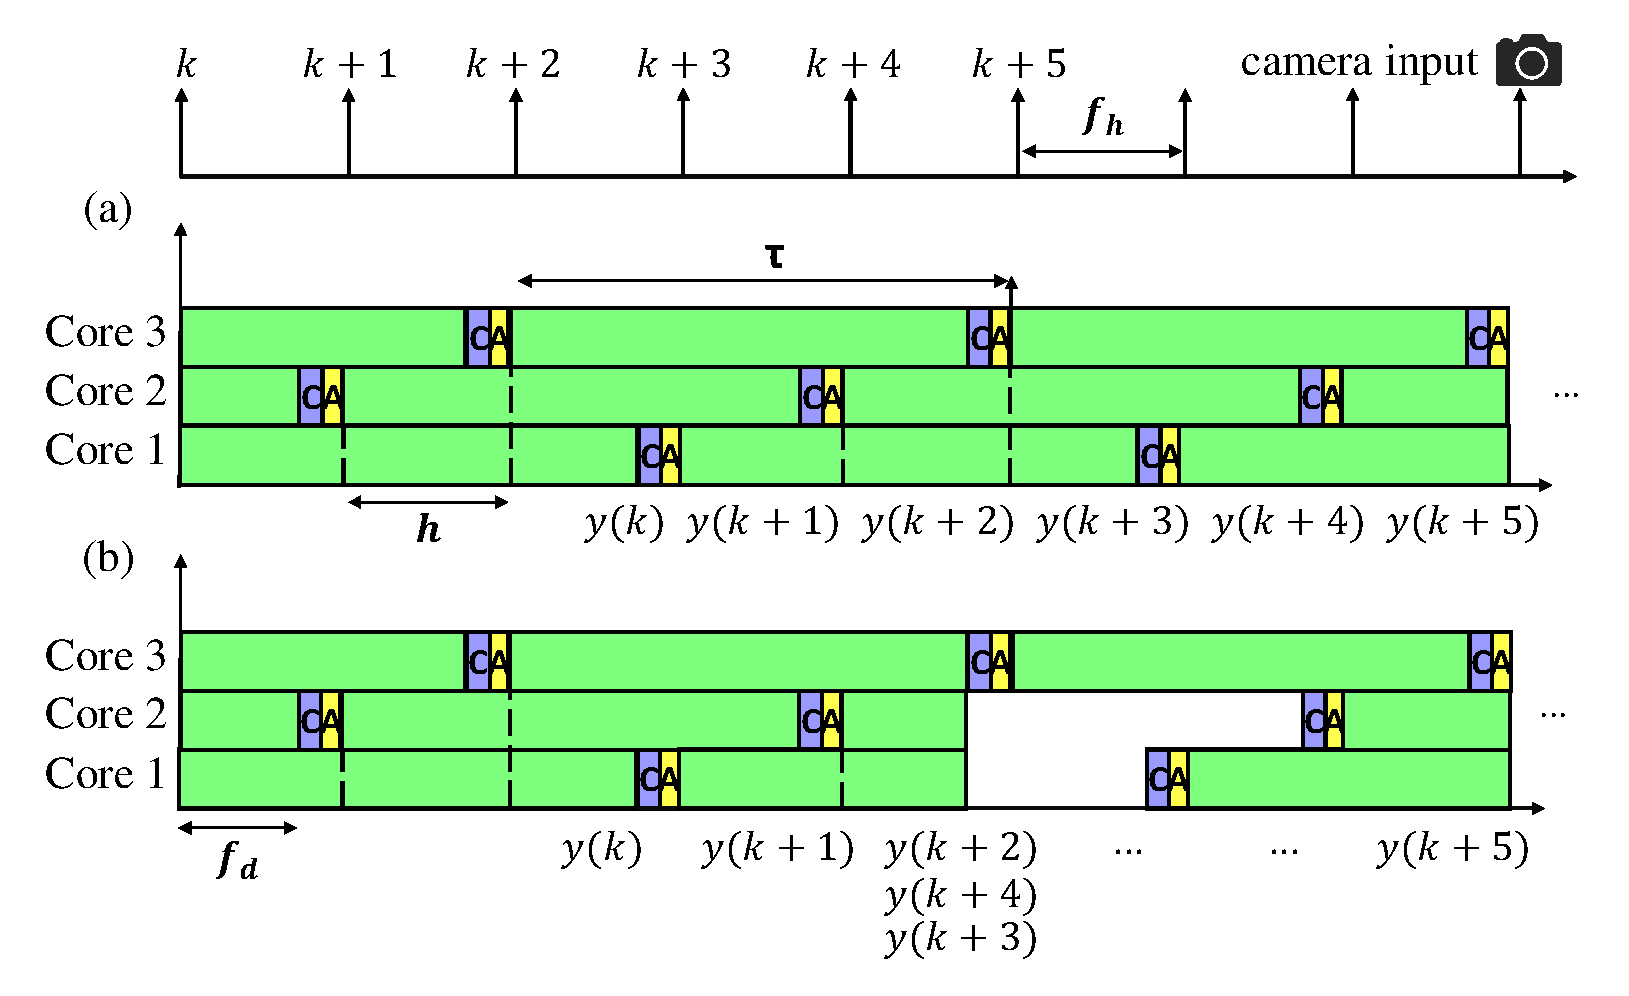
\includegraphics[width=0.9\textwidth]{images/pIBC3.eps}
    }
    \caption{Illustration of pipelined \gls{ibc} system implementation with constant sampling period $h$ and: (a) with constant worst-case sensing delay; (b) considering workload variations.}
    \label{fig:ch6_pipelined_IBC}
    \vspace{-1em}
\end{figure}

In a pipelined control implementation (see Fig.~\ref{fig:ch6_pipelined_IBC}), the
sensing operations to read and process the system states start periodically at $t_s(\taskS) = kh$, where~$k$ is a non-negative integer. 
The sampling period~$h$ is the interval between two consecutive activations of the sensing operation that require image frames for processing. 
We align $t_s(\taskS) = kh$ with the availability of the frames as can be seen in Fig.~\ref{fig:ch6_pipelined_IBC} and hence, $h$ is an integer multiple of~$\fh$.

Sensing and processing is followed by control computation and actuation operations, which generally take short and nearly constant time for execution.
A sensing operation takes much longer time due to compute heavy processing, i.e., ${\actorET_{\taskS} \gg \actorET_\taskC+\actorET_\taskA}$, where $\actorET_\taskS$, $\actorET_\taskC$ and~$\actorET_\taskA$ are the worst-case execution times of sensing and data processing, control computation and actuation tasks, respectively. 
The total (worst-case) execution time of a loop is thus given by ${\actorET_{\text{total}} = \actorET_\taskS+\actorET_\taskC+\actorET_\taskA}$. 

For a pipelined implementation, the sensor-to-actuator delay $\tau > h$ and it can be represented as~\cite{aastrom2013computer}
\begin{equation}
     \tau = (n_{f}-1)\fh+\tau_f,\text{ where } 0<\tau_f\le \fh,\ n_f =\ceil[\bigg]{\frac{\actorET_{\text{total}}}{\fh}}. \label{eq:ch6_pipe_tau}
\end{equation}
The number of frames arriving within $\tau$ is $n_f$. An assumption we make, for the scope of this chapter, is that each pipe in the pipeline is implemented on one processing core.

\section{\texorpdfstring{\Gls{spade}}{SPADe} for pipelining}
In this section, we explain the \gls{spade} approach for pipelining without parallelising the sensing task. 
The basic \gls{spade} flow for the pipelined implementation is illustrated in Fig.\ \ref{fig:ch6_spade}. A key input parameter is the total number of available cores $\numCoresAvailable$ that can be used.
We assume for now that each pipe in the pipeline is mapped to a single (unique) processing core and that there is no resource sharing between the individual pipes.
In addition, the allocated processing cores are assumed to be homogeneous so that mapping a single pipe to any of the cores would result in the same throughput and latency.
These assumptions are relaxed in Chapter \ref{chap:pipelined_parallelism}.

\begin{figure}[t]
\centerline{
    \includegraphics[width=0.7\textwidth]{images/Pipelined_SPADe.jpg}
    }
    \caption{Basic \gls{spade} flow for pipelined implementation without parallelising the sensing task. For the scope of this chapter, we assume that each pipe in the pipeline is mapped to a single (unique) processing core and the cores are homogeneous.}
    \label{fig:ch6_spade}
    \vspace{-1em}
\end{figure}
\begin{figure}[h]
\centerline{
    \includegraphics[width=0.3\textwidth]{images/pipe_sadf.jpg}
    }
    \caption{\Gls{sadf} model of a single pipe for the generic pipelined implementation. Execution time of sensing task $S$ varies per scenario.}
    \label{fig:ch6_pipe_sadf}
    \vspace{-3em}
\end{figure}
\subsection{Formal modelling and mapping}
We can model the application and the platform as explained in Section \ref{sec:ch5_MoC}.
Since there is no resource sharing between the individual pipes and each pipe is mapped to a unique processing core, we can use the generic \gls{sadf} model shown in Fig.\ \ref{fig:ch6_pipe_sadf} to compute the sensor-to-actuator delay and sampling period for a single pipe. The scenario is determined by the execution time of the sensing task S. 
When there is resource sharing between the pipes, the \gls{sadf}  model needs to be transformed for mapping and scheduling.
The model transformations are non-trivial and are explained later in Section \ref{sec:ch7_ModelTransformations}. 

\subsection{Timing analysis and system scenario identification}
The sensor-to-actuator delay for a single pipe can be computed for the generic \gls{sadf} graph illustrated in Fig. \ref{fig:ch6_pipe_sadf} using the analysis method explained in Section \ref{sec:ch5_sadf}.
We compute the best-case and worst-case sensor-to-actuator delays for the best-case and worst-case workload scenarios per pipe. The best-case workload scenario results from the shortest execution time for the sensing task and the worst-case workload scenario results from longest execution time for the sensing task.
After we compute the worst-case delay, we need to compute the effective sampling period $h$ considering the inter-frame dependencies and the platform constraints, explained below.
For the adaptive \gls{mpc} formulation-based controller design, we only need to do a runtime adaptation for considering workload variations (explained later in Section \ref{sec:ch6_cases}) and we do not need to reconfigure the mapping and scheduling (as was needed for the basic flow of the previous chapter).
This means that for the implementation proposed in this chapter, there is only one system scenario. This system scenario should know the effective period $h$, worst-case delay $\tau$, effective number of frames skipped by a single pipe $n_d$ (defined below), and the number of processing cores needed to maximise the gains from pipelining $\maxCores$ (defined below). Because of inter-frame dependencies, there is a limit on the number of cores that gives performance benefits with pipelining. 
$\tau$ is initially computed by mapping the \gls{sdf} graph of the worst-case workload scenario for a single pipe to one processing core of the given platform allocation. We can then compute the $\maxCores$ after considering the inter-frame dependencies. The effective period $h$ is then computed based on $\maxCores$ and the total number of available cores $\numCoresAvailable$. Finally, we can compute $n_d$ such that the delay $\tau$ can be expressed in multiples of the sampling period as $\tau = n_{d}h+\tau'$, where the remainder $\tau'$ is $0\leq \tau' <h$. 

\begin{figure}[t]
\centerline{
    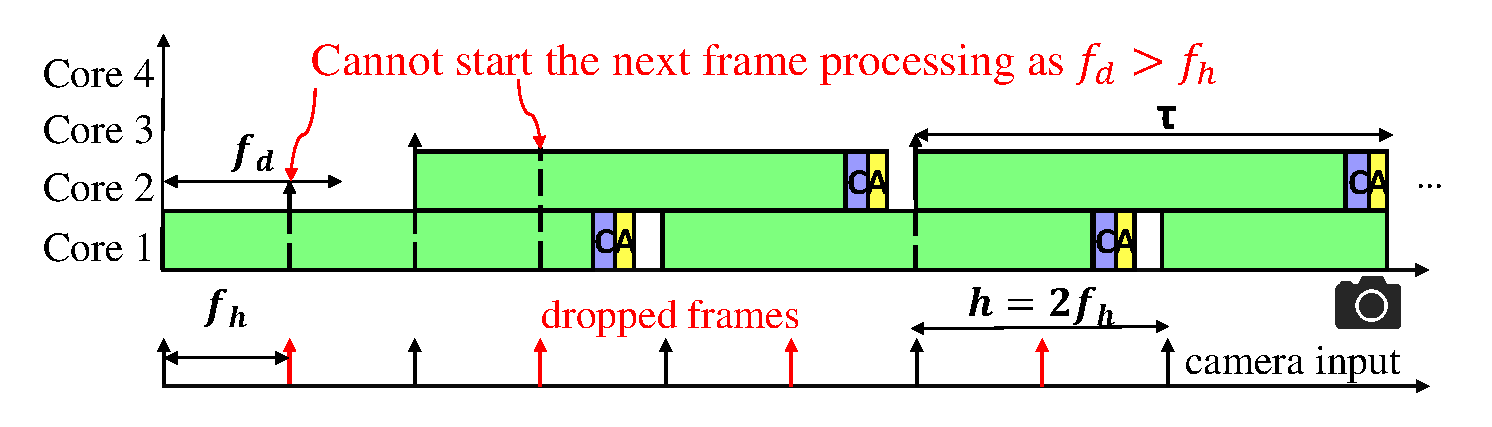
\includegraphics[width=\textwidth]{images/ifd.eps}
    }
    \caption{Illustration of inter-frame dependencies with $\fd>\fh$. Note: 1) Even if more cores are available they cannot be used due to inter-frame dependencies; 2) Our method as compared to~\cite{medina2019designing} does not restrict $\tau$ to be an integer multiple of $\fh$; 3) If $\fd\le \fh$ then $h=\fh$ using all four processing cores.}
    \label{fig:ch6_ifd}
    \vspace{-1em}
\end{figure}
\subsubsection{Adaptation with inter-frame dependencies}
\label{sec:ch6_ifd}
Inter-frame dependencies capture the data or algorithmic dependencies between consecutive frame processing.
Considering inter-frame dependencies is crucial for practical real-life implementation. 
Inter-frame dependence time $\fd$ is the maximum time required to wait between processing consecutive image frames due to inter-frame dependencies. 
Fig.~\ref{fig:ch6_ifd} illustrates the impact of inter-frame dependence time on sampling period.
In a pipelined implementation, considering inter-frame dependencies means that strictly $h\ge \fd$.
Further, $h$ should be an integer multiple of $\fh$.
For the scope of this chapter, we assume that $\fd$ is known or can be computed.
The computation of $\fd$ is explained later in Chapter \ref{chap:pipelined_parallelism}.

Inter-frame dependencies mean that sometimes some image frames have to be skipped for processing with respect to the given image arrival period $\fh$ and the sampling period $h$.
Skipping a frame means that $h$ increases and thus degrades the control performance~\cite{medina2019designing}.
The number of frames that has to be skipped after processing every frame due to inter-frame dependencies is $n_s-1$, as illustrated in Fig.~\ref{fig:ch6_ifd} where $n_s=2$ and one frame is skipped after every frame processing.
The number of frames we have to skip $n_s-1$ is determined by the inter-frame dependence time $\fd$. The earlier mentioned $n_d$ needed for defining the system scenarios is computed based on the effective $h$ and $\tau$ at runtime; we always have that $n_s\le n_d$.
$n_s$ is a constraint imposed by the inter-frame dependencies and $n_d$ is the effective number of frames we skip at runtime considering the platform constraints and $n_s$.

The effective image arrival period or the minimum possible sampling period $h_{min}$ we can then have is
\begin{equation}
    h_{min}= n_s \times \fh,\text{ where }n_s=\ceil[\bigg]{\frac{\fd}{\fh}}. \nonumber
\end{equation}
The assumption here is that a sufficient number of processing cores $\numCoresAvailable$ is available for pipelining.

\subsubsection{Adaptation with the available number of processing cores}
\label{sec:ch6_adaptation_cores}
Another crucial aspect to consider for practical implementation is the number of available processing cores.
A maximal pipelined implementation is defined as the pipelined implementation without skipping or dropping feasible image frames considering inter-frame dependencies and camera frame rate. 
A maximal pipelined implementation is achieved when the realisable periodic sampling period $h=h_{min}$. 
E.g. Fig.~\ref{fig:ch6_ifd} illustrates a maximal pipelined implementation with $n_s=2$.
The number of processing cores needed to realise the maximal pipelined implementation $\maxCores$ and the effective sampling period $h$ considering $\numCoresAvailable$ are defined as follows:
\begin{equation}
\begin{split}
    \maxCores=\ceil[\bigg]{\frac{n_f}{n_s}},\ 
        h & =\ceil[\bigg]{\frac{\maxCores}{\numCoresAvailable} n_s} \times  \fh,\ \text{if } \numCoresAvailable < \maxCores,\\
 & = n_s \times \fh,\ \text{otherwise.} \nonumber
 \end{split}
\end{equation}
where $\numCoresAvailable$ is the total number of available processing cores.
Having more cores, i.e. $\numCoresAvailable > \maxCores$, does not help as there are no more frames available for pipelining. 
However, if $\numCoresAvailable < \maxCores$, there are not enough cores available to process the arriving frames $n_f$ and thus $h$ has to be increased and a maximal pipelined implementation cannot be achieved.

\subsection{Controller design and workload variations in a pipelined \gls{ibc} system}
\label{sec:ch6_IBCworkvar}
The contribution of this chapter is the control design method using an adaptive \gls{mpc} formulation for the pipelined implementation. The controller design needs to know $h$, $\tau$ and $n_d$. The details are explained in Sections \ref{sec:ch6_modeling} and \ref{sec:ch6_MPC}.
In this section, we first analyse the impact of workload variations in a pipelined implementation.

The workload variations occur due to varying features in image content (see Fig.~\ref{fig:ch6_workload_IBC}).
When we do not consider workload variations, a pipelined implementation results in constant $\tau$ and $h$, as illustrated in Fig.~\ref{fig:ch6_pipelined_IBC}(a). 
Notice that here we measure the outputs $y(k+i)$ for the input image frame at $k+i$ with a constant worst-case sensing delay of $\tau$, where for simplicity of notation, by $k+i$ we denote the time instant $(k+i)h$ with $i$ an integer. 

Considering workload variations in a pipelined implementation of an \gls{ibc} system implies that we would have varying sensing delays, e.g., as illustrated in Fig.~\ref{fig:ch6_pipelined_IBC}(b). 
For this example, notice that the camera input frame at $k+4$ has a sensing delay of one frame ($\tau_1=h$), at $k+3$ has a sensing delay of two frames ($\tau_2=2h$) and all other frames have a sensing delay of three frames ($\tau=3h$). 
This scenario results in multiple sensing and image processing (\taskS) tasks completing their execution at the same time.
What this means is that multiple output measurements $y(k+2)$, $y(k+3)$ and $y(k+4)$ are available for control computation task $\taskC$ at the same time instance and no measurements arrive at the next two sampling instances. 

Thus, the main challenge for the pipelined \gls{ibc} system design to maximize performance, i.e. \gls{qoc}, is to effectively use the sensor measurements as early as possible for control computation without any unnecessary idling and to predict the system state when there are no sensor measurements available. Modelling this behaviour is far from trivial. 

\subsection{Runtime mechanism}
The mapping and scheduling is static at runtime for the pipelined implementation explained in this chapter.
A runtime mechanism is needed to keep track of the latest sensing measurement that is available for the \gls{mpc} computation. 
The sensing task should store the timestamp of the latest image processed and the corresponding sensing measurement in $p$ memory locations (one for each pipe).
At the start of the control compute task, the runtime mechanism needs to read the $p$ memory locations with the timestamps, compute the $n_d$ for each and choose the sensing measurement corresponding to the lowest $n_d$ value. The \gls{mpc} also requires the $n_d$ value to adapt the optimization problem formulation as explained in Section \ref{sec:ch6_cases}.
The overhead for reading the $p$ memory locations and computing $n_d$, though negligible, is part of the control compute task.